\documentclass{beamer}

\usepackage{amstext}
\usepackage{stmaryrd}
%\usepackage{listings}
%\lstset{language=C++}
%\usepackage[boxed]{algorithm2e}
\usepackage{algpseudocode}

\usepackage[normalem]{ulem}
\usepackage{graphicx}

%\usepackage{authblk}
%\usepackage{xcolor}
\usepackage{array}
\usepackage{verbatim}
\usepackage{booktabs}
\usepackage{calc}
\usepackage{textcomp}
\usepackage{multirow}
%\usepackage[boxed]{algorithm2e}

\usepackage[all]{xy}

\usepackage{cancel}
\usepackage{mathtools}
\usepackage{placeins}
\usepackage{xspace}

%\input{packages}

\usepackage{tikz,tikzscale}
\usetikzlibrary{calc}
\usetikzlibrary{shadings}
% \usepackage[backend=biber,style=alphabetic]{biblatex}
%\addbibresource{literature.bib}

%%%%%%%%%% Packages to help editing %%%%%%%%%%
%\usepackage[notref,notcite]{showkeys} % Show labels.
\usepackage[mode=multiuser,status=draft]{fixme} % Provide note, warning, error, fatal.
%\fxsetup{layout=inline}%pdfcsignote}
\fxsetup{envlayout=color}
\fxsetup{innerlayout=inline}
\fxsetup{targetlayout=colorcb}
\FXProvidesTargetLayout{color}

\fxusetheme{color}
\FXRegisterAuthor{ss}{envss}{SS}
\FXRegisterAuthor{mr}{envmr}{MR}
\FXRegisterAuthor{mw}{envmw}{MW}
\FXRegisterAuthor{mk}{envmk}{MK}

\usepackage{subcaption}
\usepackage[format=plain,indention=.5cm]{caption}
\usepackage{pgfplots}

\begin{comment}

\DontPrintSemicolon
\SetKwComment{Comment}{$\triangleleft$ }{}
\SetKwProg{Fn}{Function}{}{end}

\providecommand{\keywords}[1]
{
    \small
    \textbf{\textit{Keywords:}} #1
}
\end{comment}
% \newcommand{\FigureSubst}[1]{ \fbox{ 
% \begin{minipage} {0.7\textwidth} #1  
% \end{minipage}  }   }

\def\mesh{\mathbb M}
\def\cell{K}
\def\R{\mathbb R}
\def\ncol{N_{\text{colors}}}
\def\rest#1{I_{#1}^\downarrow}
\def\prol#1{I_{#1}^\uparrow}

\newcommand{\pluseq}{\stackrel{+}{\gets}}
%\newcommand{\pluseq}{\stackbin{+}{=}}

\newcommand{\Dd}{\text{d}}

% Mohsen's setting and definitions
%###################################%
\usepackage{bm,upgreek}
\newcommand\rd{{\rm{d}}}
\newcommand{\bfm}[1]{{\rm\bf #1}}

\newcommand{\greentext}[1]{{\color{darkgreen} #1}}
\newcommand{\bluetext}[1]{{\color{blue} #1}}
\newcommand{\redtext}[1]{{\color{red} #1}}

\DeclareMathOperator{\tr}{tr}
%###################################%

% MW settings
%###################################%

%\newcommand{\dlt}{\bm{\delta_{u}}}
%\newcommand{\corr}{\bm{{v}}}

\newcommand{\dlt}{\bm{v}}
\newcommand{\corr}{  \,\Delta \bm{u}\, }

\newcommand{\scalar }{\textit{scalar}\xspace}
\newcommand{\scalarRef}{\textit{scalar ref.}\xspace}
\newcommand{\tensorS}{\textit{tensor4}\xspace}
\newcommand{\pade}{\textit{Pade log}\xspace}
\newcommand{\none}{\textit{exact log}\xspace}
\newcommand{\tensorAD}{\textit{tensorAD}\xspace}

\newcommand{\noneSplit}{\textit{Pade root}\xspace}
\newcommand{\tensorADsplit}{\textit{tensorAD}\xspace}

\newcommand{\gz}{\mathbf{g}}

\newcommand{\Grad}{\nabla}
\newcommand{\grad}{\nabla}

\newcommand{\ds}{\,\mathrm{d}s}
\newcommand{\dx}{\,\mathrm{d}x}
%###################################%
%

\usepackage{graphicx} % Required for inserting images
\usepackage[linesnumbered,vlined,commentsnumbered,ruled]{algorithm2e}

% Avoid LaTeX failures when change-markup writes empty citation entries to the .aux
% Some change-markup writes
%    \cite  {}
% into the auxiliary files which results in an empty \citation{} entry and a
% BibTeX/LaTeX error on some toolchains. Make the redefinition defensive: only
% override \citation if it already exists, and ensure some internal citation
% helpers are defined so expansion in the .aux doesn't trigger undefined
% control sequence errors during automated builds.
\makeatletter
% Ensure internal helper \@citeb exists (some citation styles define it). If
% missing, provide a harmless empty definition to avoid "Undefined control
% sequence" when aux files contain constructs referencing it.
\providecommand\@citeb{}%

% Redefine \citation only if it exists to avoid errors when engines differ.
\@ifundefined{citation}{%
    % nothing to do: \citation not present in this format
}{%
    \let\orig@citation\citation
    \def\citation#1{%
        % Fallback check for an empty argument without relying on \@ifmtarg
        \def\@tempa{#1}%
        \ifx\@tempa\@empty
            % ignore empty citation
        \else
        \orig@citation{#1}%
        \fi
    }%
}% \@ifundefined{citation}
\makeatother
% Prevent the `changes` package from writing its local-change list to the .aux file
% (the package writes entries via \@writefile{loc}{...} which can contain
% \cite commands; those may expand into problematic empty \citation{} entries
% under some edit flows). Here we intercept writes to the "loc" stream and
% drop them while leaving other write streams intact.
\makeatletter
\let\orig@writefile\@writefile
\def\@writefile#1#2{%
    % compare the stream name to "loc"; if it matches, ignore the write
    \edef\@tempa{#1}%
    \edef\@tempb{loc}%
    \ifx\@tempa\@tempb
        % drop writes to 'loc'
    \else
    \orig@writefile{#1}{#2}%
    \fi
}
\makeatother

% \usepackage[commentmarkup,commandnameprefix=always]{changes} % For tracking revisions
\usepackage[final,commandnameprefix=always]{changes} % For tracking revisions

% Use the 'changes' package commands for revisions:
% \chadded{new text} - Marks text as added.
% \chdeleted{old text} - Marks text as deleted.
% \chreplaced{new text}{old text} - Marks text as replaced.

% horizontal strike-through using ulem (loaded above with [normalem]) 
\providecommand{\crossout}[1]{\sout{#1}}

% optional: colored strike-through (loads xcolor if not already loaded)
\usepackage{xcolor}
\providecommand{\regdel}[1]{\textcolor{blue}{\sout{#1}}}

% To control the display of changes, pass options to the package:
% \usepackage[final]{changes}    % Shows only the final version (no markup).
% \usepackage[original]{changes} % Shows only the original version (deleted text, no added text).
% \usepackage[markup=default]{changes} % Shows all changes with markup (default).
% \usepackage[commentmarkup]{changes} % Shows changes as comments in the margin.

\usepackage{amsmath,amssymb,amsfonts,graphicx,hyperref}
\usepackage{booktabs}
\usepackage{multicol}
\usepackage{tikz}
\usepackage{color}

\usetheme{default}

\usetheme{metropolis}

\titlegraphic{
    
\includegraphics[width=3cm]{Heidelberg.jpeg}}

\title{Matrix-Free Ghost Penalty Evaluation via Tensor Product Factorization}
\author{ \Large Michał Wichrowski}
\institute{ Heidelberg University}
% \date{\today}
\makeatletter
\setbeamertemplate{title page}{
    \begin{minipage}[b][\paperheight]{\textwidth}
        % \hfill \inserttitlegraphic
        %  \ifx\insertinstitute\@empty\else\usebeamertemplate*{institute}\fi
        \hfill \begin{minipage}{0.3\textwidth}
            
\includegraphics[width=\textwidth]{Heidelberg.jpeg}
            % \ifx\insertinstitute\@empty\else\usebeamertemplate*{institute}\fi
        \end{minipage}
        \vfill%
        \ifx\inserttitle\@empty\else\usebeamertemplate*{title}\fi
        \ifx\insertsubtitle\@empty\else\usebeamertemplate*{subtitle}\fi
        \usebeamertemplate*{title separator}
        \ifx\beamer@shortauthor\@empty\else{\usebeamertemplate*{author}}\fi
        \hfill	% \ifx\insertdate\@empty\else\usebeamertemplate*{date}\fi
        % \ifx\insertinstitute\@empty\else\usebeamertemplate*{institute}\fi
        \vfill
        \vspace*{1mm}
    \end{minipage}
}
\makeatother

\begin{document}

\begin{frame}
    \titlepage
\end{frame}

\begin{frame}
    \frametitle{Outline}
    \begin{itemize}
        \item Based on deal.II library
        \item CutFEM and Ghost Penalty
        \item  Factorization of Ghost Penalty Operator
        \item Matrix-free evaluation of  CutFEM Operator
        \item Numerical Results
    \end{itemize}
\end{frame}

\begin{frame}
    \frametitle{Cut FEM Discretization and Boundary Conditions}
    \textbf{Problem:} Solve $-\Delta u = f$ in $\Omega$, $u = 0$ on $\partial\Omega$.
    \begin{itemize}
        \item \textbf{Mesh:} Cartesian triangulation $\mathcal{T}_h$ with element size $h$.
        \item \textbf{FE Space:} $\mathbb{V}_h$ using Lagrange polynomial elements of order $k$.
        \item \textbf{Domain:} Level set function $\phi$ defines the discrete domain $\Omega_h$.
        \item \textbf{Weak Form:} Find $u \in \mathbb{V}_h$ such that
              \[
                  \int_{\Omega_h} \nabla u \cdot \nabla v \dx = \int_{\Omega_h} f v \dx \quad \forall v \in
                  \mathbb{V}_h.
              \]
        \item \textbf{Nitsche's Method:} Weakly enforce Dirichlet boundary conditions with
              \[
                  \int_{\partial\Omega_h} \left( \frac{\partial u}{\partial n} v + \frac{\partial v}{\partial n} u +
                  \gamma_D u v \right) \ds,
              \]
              where \( \gamma_D = 30 k (k+1) \) for stability.
    \end{itemize}
\end{frame}

\begin{frame}
    \frametitle{Ghost Penalty Stabilization}
    \begin{itemize}
        \item Penalizes discontinuities across element faces cut by the boundary.
        \item
              \(
              g_h(u_h,v_h) = \gamma_A \sum_{F \in \mathcal{F}_h} g_F(u_h, v_h),
              \)
        \item
              \(
              g_F(u_h, v_h) = \gamma_A \sum_{k=0}^p \left(\frac{h_F^{2k-1}}{k!^2}[\partial_n^k u_h],
              [\partial_n^k v_h]
              \right)_F
              \)
        \item $\mathcal{F}_h$: set of all interior faces of intersected cells
    \end{itemize}
    \begin{center}
        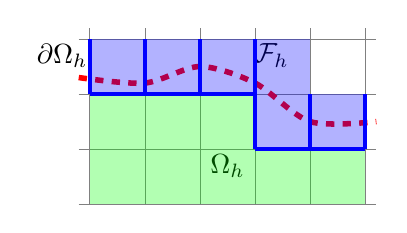
\begin{tikzpicture}[scale=0.7]
            % Draw the Cartesian grid
            \draw[step=1cm, gray, very thin] (-0.2,0) grid (5.2,3.2);

            % Draw the curved interface
            \node at (-0.5,2.7) {$\partial\Omega_h$};
            \draw[line width=2pt, red, dashed] plot [smooth, tension=0.5] coordinates {(-0.2,2.3) (1,2.2)
                    (2,2.5) (3,2.2)
                    (4,1.5)
                    (5.2,1.5)};

            \node at (2.5,0.7) {$\Omega_h$};
            \node at (3.3,2.7) {$\mathcal{F}_h$};

            % Highlight intersected cells
            \foreach \x/\y in {0/2, 1/2, 2/2, 3/1, 3/2, 4/1}
                {
                    \fill[blue, opacity=0.3] (\x,\y) rectangle (\x+1,\y+1);
                }
            % Highlight cells inside the domain
            \foreach \x/\y in {0/0, 0/1,2/1, 1/0, 1/1, 2/0, 3/0, 4/0}
                {
                    \fill[green, opacity=0.3] (\x,\y) rectangle (\x+1,\y+1);
                }

            % Highlight the edges between intersected and non-intersected cells
            \foreach \x/\y in {0/2, 1/2, 2/2, 2/1, 3/1 , -1/2, 4/1 } {
                    \draw[blue, line width=1.5pt] (\x+1,\y) -- (\x+1,\y+1);
                };

            \foreach \x/\y in {0/1, 1/1, 2/1		/	,	3/0, 4/0 } {
                    \draw[blue, line width=1.5pt] (\x,\y+1) -- (\x+1,\y+1);
                };

        \end{tikzpicture}
    \end{center}
\end{frame}

\begin{frame}
    \frametitle{Tensor Product Structure}
    \begin{itemize}
        \item Multiindex notation: $i = (i_1, i_2, i_3)$
        \item Basis functions are products of 1D functions:
              \[
                  \phi_{i}( x ) = \phi_{i_1}(x_{1}) \cdot \phi_{i_2}(x_{2}) \cdot
                  \phi_{i_3}(x_{3}).
              \]
        \item Values of function \( u \) at a given point:
              \[
                  u (x) = \sum_{i_1, i_2, i_3} u_{i_1 i_2 i_3} \phi_{i_1}(x_{1}) \cdot \phi_{i_2}(x_2) \cdot
                  \phi_{i_3}(x_3)
              \]
    \end{itemize}
    \begin{center}
        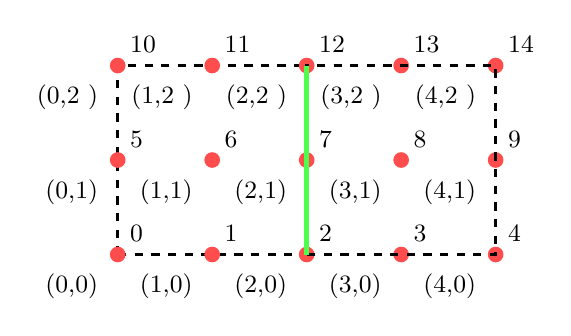
\begin{tikzpicture}[scale=1.2]
            % Cell 1
            \draw[line width=1pt, dashed] (-2,0) rectangle (0,2) node[midway, below] {
                    % $K_1$
                };
            \foreach \x in {0,1,2,3, 4}
            \foreach \y in {0,1,2 }
            {
            \node[circle,inner sep=2pt,fill=red!70,label={[label distance=2pt]below left:{\small (\x,\y)}}]
            (K1-\x-\y) at (-2+\x*2/2,\y*2/2) {};
            \pgfmathtruncatemacro{\index}{\x + \y * 5}
            \node[above right=1pt,font=\small] at (K1-\x-\y) {\index};
            }

            % Cell 2
            \draw[line width=1pt, dashed] (0,0) rectangle (2,2) node[midway, below] {
                    % $K_2$
                };

            % Face F
            \draw[line width=2pt, green!70] (0,0) -- (0,2) node[midway, right, below, black] {
                % $\; \;\; F$
            };

        \end{tikzpicture}
    \end{center}
\end{frame}

\begin{frame}
    \frametitle{Ghost Penalty Matrix Derivation}
    \begin{itemize}
        \item Local penalty matrix $\mathcal{G}_{F,k}$:
              \[
                  [\mathcal{G}_{F,k} ]_{i,j} = \left( [\partial_n^k \phi_j], [\partial_n^k \phi_i] \right)_F.
              \]
        \item Expanding shape functions:
              \begin{align*}
                  [\mathcal{G}_{F,k} ]_{i,j} & = \left( [\partial_n^k \phi_{j_1}] \cdot \phi_{j_2}\phi_{j_3},
                  [\partial_n^k \phi_{i_1}] \cdot \phi_{i_2}\phi_{i_3} \right)_F                              \\
                                             & =	[\partial_n^k \phi_{i_1}]_{F} \cdot [\partial_n^k
                      \phi_{j_1}]_{F}	\cdot
                  \Bigl( \phi_{i_2}\phi_{i_3} , \phi_{j_2}\phi_{j_3} \Bigr)_F
              \end{align*}
        \item 1D ghost penalty term:
              \[
                  [G^h_k]_{i_1,j_1} = \left[\partial_n^k \phi_{i_1}\right]_{F} \, \left[\partial_n^k
                      \phi_{j_1}\right]_{F}.
              \]
        \item 1D mass matrices:
              \[
                  M^{2,h }_{i_2,j_2} = \Bigl( \phi_{i_2} , \phi_{j_2} \Bigr)_{F_2}, \quad
                  M^{3,h}_{i_3,j_3} = \Bigl( \phi_{i_3} , \phi_{j_3} \Bigr)_{F_3}.
              \]
    \end{itemize}
\end{frame}

\begin{frame}
    \frametitle{Kronecker Product Structure}
    \begin{itemize}
        \item Ghost penalty matrix as Kronecker product:
              \[
                  \mathcal{G}_{F,k} = M^{h} \otimes M^{h} \otimes G^h_k .
              \]
        \item Matrices are scaled with mesh size $h$.
        \item Precompute scaled mass matrix  $h M^1$ and scaled penalty matrix
              \[
                  G^1 = \sum_{k=0}^p \left( { h^{-1} k!^{-2}} G^1_k \right).
              \]
              The scaling comes from the following derivation:
              \begin{align*}
                  [G^h_k]_{i_1,j_1} & = \left[\partial_n^k \phi_{i_1}\right]_{F}\cdot \left[\partial_n^k
                      \phi_{j_1}\right]_{F}
                  =  \left[{1\over h^k} \partial_n^k \phi^{\text{ref}}_{i_1}\right] _{\hat{F}} \cdot \left[{1\over h^k}
                      \partial_n^k \phi^\text{ref}_{j_1}\right]_{\hat{F}}
                  \nonumber
                  \\
                                    & = {1\over h^{2k}} \left[\partial_n^k
                      \phi^{\text{ref}}_{i_1}\right]_{\hat{F}}\cdot
                  \left[\partial_n^k \phi^{\text{ref}}_{j_1}\right]_{\hat{F}}= {1\over h^{2k}} [G^1_k]_{i_1,j_1}.
              \end{align*}
    \end{itemize}
\end{frame}

\begin{frame}
    \frametitle{Ghost Penalty Matrix and Application}
    \begin{itemize}
        \item Ghost penalty matrix as Kronecker product (face orthogonal to $x_1$):
              \[
                  \mathcal{G}_{F,k} = M^{h} \otimes M^{h} \otimes G^h_k .
              \]
        \item Complete ghost penalty matrix:
              \begin{align*}
                  \mathcal{G}_F & = \gamma_A \sum_{k=0}^p \frac{h_F^{2k-1}}{k!^2} \left( M^h \otimes M^h \otimes
                  G^h_k
                  \right)                                                                                        \\
                                & = \gamma_A \; h M^1 \otimes h M^1 \otimes	\sum_{k=0}^p \left( { h^{-1} k!^{-2}}
                  G^1_k
                  \right).
              \end{align*}
    \end{itemize}
\end{frame}

\begin{frame}
    \frametitle{Application of the Ghost Penalty Operator}
    \begin{itemize}
        \item Contribution of the face $F$ to the vector $w$:
              \(
              w_F =  \gamma_A  h^{2} M^h \otimes M^h \otimes G^1	\cdot u.
              \)
        \item Decomposed into a sequence of matrix-vector products:
              \begin{align*}
                  w_F^1 & =  \gamma_A \;  I \otimes I \otimes G^1 \cdot u          \\
                  w_F^2 & =  \gamma_A \;  I \otimes h M^1 \otimes I \cdot w_F^{1}, \\
                  w_F   & =  \gamma_A \; h M^1 \otimes I \otimes I \cdot w_F^{2}.
              \end{align*}
        \item Cost per face: $O((2k+1)^2 (k+1)^{d-1}) $.
    \end{itemize}
\end{frame}

\begin{frame}
    \frametitle{Treatment of Internal and Intersected Cells}
    \begin{itemize}
        \item \textbf{Internal Cells:}
              \begin{itemize}
                  \item Local contribution:
                        \[
                            w_{Ki}=\int\limits_K	\nabla u_K   \cdot \nabla {\phi }_i \;	\Dd x
                            = \sum_{q(K)} \nabla u_K   \cdot  \nabla\phi_i \, J(x_q) \,
                            \omega_q.
                        \]
                  \item Sum factorization to reduce the cost of evaluating gradients and integrating.
                  \item Complexity: $\mathcal{O}((k+1)^{d+1}) = \mathcal{O}((k+1)     N_c)$.
              \end{itemize}
        \item \textbf{Intersected Cells:}
              \begin{itemize}
                  \item Integration performed only over the part of the cell inside the domain $\Omega$.
                  \item Quadrature formula generated according to~\textcolor{blue}{[Saye2015]}.
                  \item Store locations of quadrature points, Jacobian matrices, integration weights, and normal
                        vectors.
                  \item No sum factorization for intersected cells.
                  \item Implementation	\textcolor{blue}{[Bergbauer2024]}
              \end{itemize}
    \end{itemize}
\end{frame}

\begin{frame}
    \frametitle{Convergence: sanity check}
    \begin{itemize}
        \item Domain $\Omega$: interior of the unit ball.
        \item Uniform Cartesian mesh $\mathcal{T}_h$.
        \item Poisson problem with zero Dirichlet boundary conditions.
        \item Conjugate gradient method with a relative tolerance of $10^{-8}$.
    \end{itemize}
    \begin{center}
        \begin{tikzpicture}
            \begin{axis}[
                    ylabel=\(L^2\) Error,
                    xmode=log,
                    ymode=log,
                    legend pos=outer north east,
                    width=0.8\textwidth,
                    height=0.5\textwidth,
                    grid=both,
                    minor tick num=1,
                    log basis x=10,
                    log basis y=10,
                    xtick={0.0164,0.0328,0.0656,0.1312,0.2625,0.5250,1.0500},
                    ytick={1e-8,1e-7,1e-6,1e-5,1e-4,1e-3,1e-2,1e-1,1},
                    xticklabels={$2^{-3}h_0$,,$2^{-2}h_0$,,$2^{-1}h_0$,, $h_0$},
                    yticklabels={,1e-7,,1e-5,,1e-3,,1},
                    xmin=0.011,
                    xmax=1.1,
                    ymin=1e-8,
                    ymax=1.1,
                ]

                \addplot[color=blue, mark=o, mark size=3pt, line width=1pt] table [x index=1, y index=2,header=has
                        colnames]
                    {results/convergence_2d_d1.txt};
                \addlegendentry{\(k=1\)}

                \addplot[color=red, mark=x, mark size=3pt, line width=1pt] table [x index=1, y index=2, header=has
                        colnames]
                    {results/convergence_2d_d2.txt};
                \addlegendentry{\(k=2\)}

                \addplot[color=green, mark=+, mark size=3pt, line width=1pt] table [x index=1, y index=2, header=has
                        colnames]
                    {results/convergence_2d_d3.txt};
                \addlegendentry{\(k=3\)}

                \addplot[color=blue, dashed, domain=0.01:1, samples=3, variable=\x] {0.5*\x^2};
                \addplot[color=red, dashed, domain=0.01:1, samples=3, variable=\x] {0.02*\x^3};
                \addplot[color=green, dashed, domain=0.01:1, samples=3, variable=\x] {0.001*\x^4};

            \end{axis}
        \end{tikzpicture}
    \end{center}
\end{frame}

\begin{frame}
    \frametitle{Computational Efficiency}
    \begin{itemize}
        \item Benchmark the computational cost of the Laplacian operator on a single cell in 2D and 3D.
        \item Compare three approaches:
              \begin{itemize}
                  \item FEEvaluation: Standard matrix-free evaluation exploiting tensor product factorization.
                  \item FEPointEvaluation: without  tensor product factorization.
                  \item GhostPenalty: Ghost penalty evaluation on one face.
              \end{itemize}
    \end{itemize}
\end{frame}

\begin{frame}
    \frametitle{Single Cell Performance}
    Benchmark the computational cost of the Laplacian operator
    \begin{columns}
        \begin{column}{0.5\textwidth}
            \centering
            \begin{tikzpicture}
                \begin{axis}[
                        xlabel=Degree,
                        ylabel=Relative timing,
                        % legend pos=outer north east,
                        width=\textwidth,
                        height=\textwidth,
                        grid=both,
                        ymode=log,
                        log basis y=2,
                        ymin =0.60,
                        title=2D,
                    ]
                    \addplot[color=blue, mark=o, mark size=3pt, line width=1pt] table [x index=0, y
                            index=1, y expr=\thisrowno{1}*8/(7.7400e-02), header=has
                            colnames]
                        {results/one_cell_2d.txt};
                    % \addlegendentry{FEPointEval}

                    \addplot[color=red, mark=x, mark size=3pt, line width=1pt] table [x index=0, y
                            index=2,  y expr=\thisrowno{2}/(7.7400e-02), header=has
                            colnames]
                        {results/one_cell_2d.txt};
                    % \addlegendentry{FEEvaluation}

                    \addplot[color=green, mark=+, mark size=3pt, line width=1pt] table [x index=0, y
                            expr=\thisrowno{3}/(7.7400e-02),
                            header=has
                            colnames]
                        {results/one_cell_2d.txt};
                    % \addlegendentry{GhostPenalty}

                \end{axis}
            \end{tikzpicture}
            % \caption{2D}
        \end{column}
        \begin{column}{0.5\textwidth}
            % \begin{figure}
            \centering
            \begin{tikzpicture}
                \begin{axis}[
                        xlabel=Degree,
                        title=2D,
                        legend pos=north west,
                        width=\textwidth,
                        height=\textwidth,
                        grid=both,
                        ymode=log,
                        log basis y=2,
                        ymin =0.55,
                        ymax = 0.5e5
                    ]
                    \addplot[color=blue, mark=o, mark size=3pt, line width=1pt] table [x index=0, y
                            index=1, y expr=\thisrowno{1}*8/(2.2180e-01), header=has
                            colnames]
                        {results/one_cell_3d.txt};
                    % \addlegendentry{FEPointEval}

                    \addplot[color=red, mark=x, mark size=3pt, line width=1pt] table [x index=0, y
                            index=2,  y expr=\thisrowno{2}/(2.2180e-01), header=has
                            colnames]
                        {results/one_cell_3d.txt};
                    % \addlegendentry{FEEval}

                    \addplot[color=green, mark=+, mark size=3pt, line width=1pt] table [x index=0,
                            y
                            expr=\thisrowno{3}/(2.2180e-01),
                            header=has
                            colnames]
                        {results/one_cell_3d.txt};
                    % \addlegendentry{GhostPenalty}

                \end{axis}
            \end{tikzpicture}
            % \caption{3D}
            % \end{figure}
        \end{column}
    \end{columns}
    \vspace{-1em}
    \begin{center}
        \hspace{3em }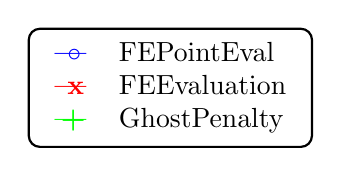
\begin{tikzpicture}
            \node[anchor=west, draw=black, thick, rectangle, rounded corners] at (0,0) {
                \begin{tabular}{ll}
                    \textcolor{blue}{\textbf{---\hspace{-0.6em}$\circ$}} & FEPointEval  \\
                    \textcolor{red}{\textbf{---\hspace{-0.6em}x}}        & FEEvaluation \\
                    \textcolor{green}{\textbf{---\hspace{-0.8em}+}}      & GhostPenalty
                \end{tabular}
            };
        \end{tikzpicture}
    \end{center}
\end{frame}

% \begin{frame}
%     \frametitle{Matrix-free vmult 2D}
%     \begin{itemize}
%         \item Time required for a single matrix-vector multiplication (vmult) per unknown.
%         \item Time per degree of freedom decreases with increasing polynomial degree.
%     \end{itemize}
%     \begin{center}
%         \begin{tikzpicture}
%             \begin{axis}[
%                     xlabel={Number of Degrees of Freedom},
%                     ylabel={Time per vmult [seconds]},
%                     xmode=log,
%                     ymode=log,
%                     legend pos=outer north east,
%                     width=0.8\textwidth,
%                     height=0.5\textwidth,
%                     grid=both,
%                     minor tick num=1,
%                     log basis x=10,
%                     log basis y=10,
%                 ]

%                 \addplot[color=blue, mark=o, mark size=3pt, line width=1pt] table [
%                         x index=2,
%                         y expr=\thisrowno{2}/\thisrowno{3}*1e3,
%                         header=has colnames]
%                     {results/vmult_single_2D_d1.txt};
%                 \addlegendentry{\(k=1\)}

%                 \addplot[color=red, mark=x, mark size=3pt, line width=1pt] table [
%                         x index=2,
%                         y expr=\thisrowno{2}/\thisrowno{3}*1e3,
%                         header=has colnames]
%                     {results/vmult_single_2D_d2.txt};
%                 \addlegendentry{\(k=2\)}

%                 \addplot[color=green, mark=+, mark size=3pt, line width=1pt] table [
%                         x index=2,
%                         y expr=\thisrowno{2}/\thisrowno{3}*1e3,
%                         header=has colnames]
%                     {results/vmult_single_2D_d3.txt};
%                 \addlegendentry{\(k=3\)}

%             \end{axis}
%         \end{tikzpicture}
%     \end{center}
% \end{frame}

\begin{frame}
    \frametitle{Matrix-free vmult 3D}

    \begin{itemize}
        \item  $\Omega$: interior of the unit ball.
        \item Time required for a single matrix-vector multiplication (vmult) per unknown.
        \item Time per degree of freedom decreases with increasing polynomial degree.
    \end{itemize}
    \begin{center}
        \begin{tikzpicture}
            \begin{axis}[
                    xlabel={Number of Degrees of Freedom},
                    ylabel={Time per vmult [seconds]},
                    xmode=log,
                    ymode=log,
                    legend pos=outer north east,
                    width=0.8\textwidth,
                    height=0.5\textwidth,
                    grid=both,
                    minor tick num=1,
                    log basis x=10,
                    log basis y=10,
                ]

                \addplot[color=blue, mark=o, mark size=3pt, line width=1pt] table [
                        x index=2,
                        y expr=\thisrowno{2}/\thisrowno{3}*1e3,
                        header=has colnames]
                    {results/vmult_single_3D_d1.txt};
                \addlegendentry{\(k=1\)}

                \addplot[color=red, mark=x, mark size=3pt, line width=1pt] table [
                        x index=2,
                        y expr=\thisrowno{2}/\thisrowno{3}*1e3,
                        header=has colnames]
                    {results/vmult_single_3D_d2.txt};
                \addlegendentry{\(k=2\)}

                \addplot[color=green, mark=+, mark size=3pt, line width=1pt] table [
                        x index=2,
                        y expr=\thisrowno{2}/\thisrowno{3}*1e3,
                        header=has colnames]
                    {results/vmult_single_3D_d3.txt};
                \addlegendentry{\(k=3\)}

            \end{axis}
        \end{tikzpicture}
    \end{center}
\end{frame}

\begin{frame}
    \frametitle{Time Breakdown: multiple balls domain}
    \begin{itemize}
        \item 3D problem with $k=3$, 26\% cut cells, 6,129,445 DoFs.
        \item Cut cells consume the most time followed by the ghost penalty term.
    \end{itemize}
    \begin{center}
        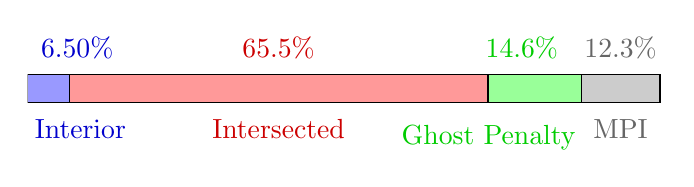
\begin{tikzpicture}
            \begin{axis}[
                    xbar stacked,
                    xmin=0, xmax=100,
                    xlabel={Percentage of Total vmult Time},
                    width=0.8\textwidth,
                    height=0.3\textwidth,
                    ytick=\empty,
                    axis lines=none
                ]
                \addplot[fill=blue!40, draw=black, line width=0.5pt] coordinates {(6.50,0)};
                \node at (axis cs:15.50/2,0.5) [blue!80!black]
                {6.50\%};
                \node at (axis cs:16.50/2,-0.5) [blue!80!black] {Interior};

                \addplot[fill=red!40, draw=black, line width=0.5pt] coordinates {(65.5,0)};
                \node at (axis cs:6.50 + 65.5/2,0.5) [red!80!black]
                {65.5\%};
                \node at (axis cs:6.50 + 65.5/2,-0.5) [red!80!black]
                {Intersected};

                \addplot[fill=green!40, draw=black, line width=0.5pt] coordinates {(14.6,0)};
                \node at (axis cs:6.50 + 65.5 + 10.6/2,0.5)
                [green!80!black] {14.6\%};
                \node at (axis cs:6.50 + 65.5 + 0.2/2,-0.6)
                [green!80!black] {Ghost Penalty};

                \addplot[fill=gray!40, draw=black, line width=0.5pt] coordinates {(12.3,0)};
                \node at (axis cs:6.50 + 65.5 + 14.6 + 12.3/2,0.5)
                [gray!80!black] {12.3\%};
                \node at (axis cs:6.50 + 65.5 + 14.6 + 12.3/2,-0.5)
                [gray!80!black] {MPI};

            \end{axis}
        \end{tikzpicture}
    \end{center}
    \begin{center}
        \includegraphics[width=0.5\textwidth]{figs/balls.pdf}
    \end{center}
\end{frame}

\begin{frame}
    \frametitle{Matrix-free vmult 3D: multiple balls}

    \begin{itemize}
        \item  $\Omega$: multiple balls.
        \item Time required for a single matrix-vector multiplication (vmult) per unknown.
        \item Performance deteriorates with increasing number of intersected cells.
    \end{itemize}
    \begin{center}
        \begin{tikzpicture}
            \begin{axis}[
                    xlabel={Intersected cells fraction},
                    ylabel={DoF per second},
                    xmode=linear,
                    ymode=log,
                    xmax=0.3,
                    legend pos= north east,
                    width=0.8\textwidth,
                    height=0.5\textwidth,
                    grid=both,
                    minor tick num=1,
                    % log basis x=10,
                    log basis y=10,
                ]

                \addplot[color=blue, mark=o, mark size=3pt, line width=1pt] table [
                        x index=10,
                        y expr=\thisrowno{3}/\thisrowno{4},
                        header=has colnames]
                    {results/vmult_multiple_3D_d1_alt.txt};
                \addlegendentry{\(k=1\)}

                \addplot[color=red, mark=x, mark size=3pt, line width=1pt] table [
                        x index=10,
                        y expr=\thisrowno{3}/\thisrowno{4},
                        header=has colnames]
                    {results/vmult_multiple_3D_d2_alt.txt};
                \addlegendentry{\(k=2\)}

                \addplot[color=green, mark=+, mark size=3pt, line width=1pt] table [
                        x index=10,
                        y expr=\thisrowno{3}/\thisrowno{4},
                        header=has colnames]
                    {results/vmult_multiple_3D_d3_alt.txt};
                \addlegendentry{\(k=3\)}

            \end{axis}
        \end{tikzpicture}
    \end{center}
\end{frame}

\begin{frame}
    \frametitle{Conclusion}
    \begin{itemize}
        \item Matrix-free approach to implement and evaluate the ghost penalty technique for CutFEM.
        \item Avoids the assembly of global matrices.
        \item Evaluation reduces to a series of precomputed 1D matrix-vector products.
        \item No need to integrate high order derivatives.
    \end{itemize}
\end{frame}

\end{document}